\documentclass[12pt,a4paper]{article}
\usepackage{verbatim}
\usepackage{graphicx}
\usepackage{amsmath}
\usepackage{float}
\author{ZHANG Xiao Research Intern in IBM CRL}
\title{Network 20q HW7}

\begin{document}
\maketitle
\pagebreak

\section{Time-Dependent Pricing}
In this question, we need to calculate the optimal reward for the data delay transmission.

The proportions of delay transmission data is:
\begin{equation}
w_A(p) = 1 - e^{-\frac{p}{4}}
\end{equation}
\begin{equation}
w_B(p) = 1 - e^{-\frac{p}{2}}
\end{equation}

So the volume of transmitted data for A is:
\begin{equation}
v_{A,day}*w_A(p) = 8*(1 - e^{-\frac{p}{4}})
\end{equation}

The volume of transmitted data for B is:
\begin{equation}
v_{B,day}*w_B(p) = 6*(1 - e^{-\frac{p}{2}})
\end{equation}

The total cost for the reward is:
\begin{equation}
C_{reward} = p*(8*(1 - e^{-\frac{p}{4}}) +  6*(1 - e^{-\frac{p}{2}}) )
\end{equation}

At the same time, the exceeding costs for day time and night time are:
\begin{equation}
C_{night} = max\{5+8*(1 - e^{-\frac{p}{4}}) + 6*(1 - e^{-\frac{p}{2}}) - 10, 0\}
\end{equation}

\begin{equation}
C_{day} = max\{4-8*(1 - e^{-\frac{p}{4}}) - 6*(1 - e^{-\frac{p}{2}}) , 0\}
\end{equation}

So the object function is:
\begin{equation}
C_{reward} + C_{day} + C_{night}
\end{equation}

We need to extract the optimal $p^{*}$, to make the object function minimal.

With the source code in python, we could get the plot of cost v.s. the reward $p$, from the graph, we could conclude that, the function is a convex function.

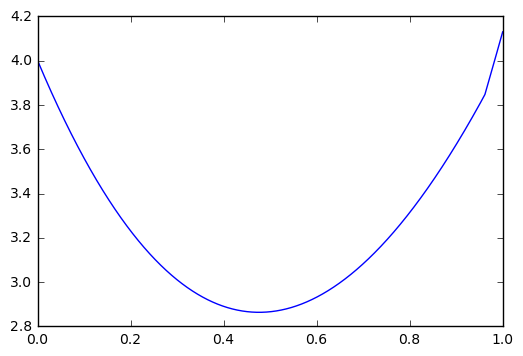
\includegraphics{PIC/cost.png}

And we could get the numerical solution by differentiate the cost function, by finding the first positive element, we could get the $p^*$.

\begin{equation}
p^* = 0.47614761476147616
\end{equation}

\section{RIP}

\subsection{a}
At the beginning, $t=0$, each node could only see itself


\begin{equation}
\begin{tabular}{ l l l l }
\hline
Node & Destination & Cost & Next \\
\hline
 A & A & 0 & A\\
 B & B & 0 & B\\
 C & C & 0 & C\\
 D & D & 0 & D\\
\hline
\end{tabular}
\end{equation}

When $t=1$:
\begin{equation}
\begin{tabular}{ l l l l }
\hline
Node & Destination & Cost & Next \\
\hline
 A & C & 2 & A\\
\hline
 B & C & 1 & B\\
 B & D & 6 & B\\
\hline
 C & D & 3 & C\\
 C & A & 2 & C\\
 C & B & 1 & C\\
\hline
D & B & 6 & C\\
D & C & 3 & C\\
\hline
\end{tabular}
\end{equation}
When $t=2$:
\begin{equation}
\begin{tabular}{ l l l l }
\hline
Node & Destination & Cost & Next \\
\hline
 A & B & 3 & C\\
 A & C & 2 & A\\
 A & D & 5 & C\\
\hline
 B & A & 3 & C\\
 B & C & 1 & B\\
 B & D & 4 & C\\
\hline
 C & A & 2 & C\\
 C & B & 1 & C\\
 C & D & 3 & C\\
\hline
 D & A & 5 & C\\
 D & B & 4 & C\\
 D & C & 3 & C\\
\hline
\end{tabular}
\end{equation}

\subsection{b}

While the link A to C failed, and B, C update the table, C would clean current path, and update its route with the link with B ,we could get:

\begin{equation}
\begin{tabular}{ l l l l }
\hline
Node & Destination & Cost & Next \\
\hline
 B & A & 3 & C\\
 C & A & 4 & B\\
 D & A & 5 & C\\
\hline
\end{tabular}
\end{equation}

Then B and D have to update
\begin{equation}
\begin{tabular}{ l l l l }
\hline
Node & Destination & Cost & Next \\
\hline
 B & A & 5 & C\\
 C & A & 4 & B\\
 D & A & 7 & C\\
\hline
\end{tabular}
\end{equation}

Then C would update again with C to B
\begin{equation}
\begin{tabular}{ l l l l }
\hline
Node & Destination & Cost & Next \\
\hline
 B & A & 5 & C\\
 C & A & 6 & B\\
 D & A & 7 & C\\
\hline
\end{tabular}
\end{equation}

The weight of path would increase to $\infty$

\subsection{c}

We could adopt the norms of many routing protocols that forbid the update coming back from last hop, which means do not allow update information coming back from a newly updated one.



\end{document}